%-------------------------------------------------
%	Version: 0.0
%	fecha de entrega
%
%-------------------------------------------------

\documentclass[11pt]{report}

%packages
\usepackage{graphicx}
\usepackage{subcaption}

\usepackage[utf8]{inputenc}
\usepackage[spanish, es-nodecimaldot]{babel}
\usepackage{setspace}
\usepackage{ragged2e}

\usepackage{amsmath}
\usepackage{amsthm}
\usepackage{amssymb}
\usepackage{mathtools}
\usepackage{siunitx}
\usepackage[thinc]{esdiff} %derivadas faciles
\usepackage{physics} %algunos simbolos de derivadas

%path donde se encuentran las imagenes
\graphicspath{ {./figuras/} }

%---------------------------------------------------------------
%ABREVIACIONES DE COMANDOS

\theoremstyle{plain}
\newtheorem{thm}{Teorema}[chapter] % reset theorem numbering for each chapter

\theoremstyle{definition}
\newtheorem{defn}[thm]{Definición} % definition numbers are dependent on theorem numbers
\newtheorem{exmp}[thm]{Ejemplo} % same for example numbers

\newcommand{\chaptercontent}{
\section{Basics}
\begin{defn}Here is a new definition.\end{defn}
\begin{thm}Here is a new theorem.\end{thm}
\begin{thm}Here is a new theorem.\end{thm}
\begin{exmp}Here is a good example.\end{exmp}
\subsection{Some tips}
\begin{defn}Here is a new definition.\end{defn}
\section{Advanced stuff}
\begin{defn}Here is a new definition.\end{defn}
\subsection{Warnings}
\begin{defn}Here is a new definition.\end{defn}
}

\usepackage{biblatex}
%\addbibresource{Tarea1.bib}

\begin{document}

\begin{titlepage}
\title{Titulo_del_trabajo}

%-------------------------------------------------
%PORTADA
%-------------------------------------------------

	\centering
	{\scshape\LARGE Universidad Autónoma de Yucatán  \\ Facultad de ingeniería\par}
	\vspace{1cm}
	{\scshape\Large Teoría electromagnética II\par}
	\vspace{1.5cm}
	{\huge\bfseries Apuntes de clase\par}
	\vspace{0.7cm}
	{\begin{figure}[!h]
	\centering
    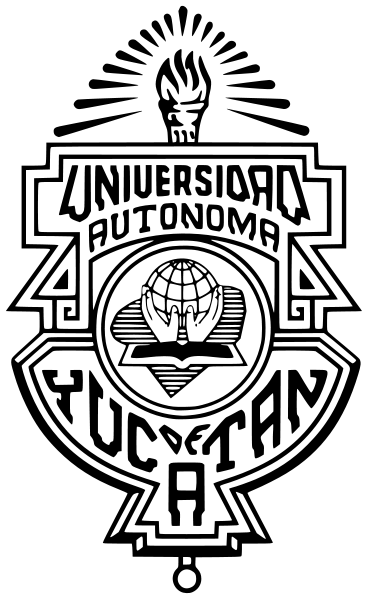
\includegraphics[scale=0.3]{UADY.png}
	\end{figure}}
	\vspace{0.7cm}
	{\Large\itshape Erick Al. Casanova Cortés\par}
	{\Large\itshape Matricula: 15014866\par}
	\vfill
	{\scshape\Large Docente\par
	Dr. O. Carvente\par}
	\vfill
	{\Large{\bfseries Fecha de modificación: \today} }

	\vfill
	
\end{titlepage}

%-------------------------------------------------
%Inicio del documento
%-------------------------------------------------

\tableofcontents

%-------------------------------------------------
%Introducción
%-------------------------------------------------

\chapter{Introducción}
\section{Formativa y sumativa}
ADAs 40 \% \\
Examenes 60 \% \\


\subsection{ADAs}
Reporte, portada, introducción, metodología, conclusiones y bibliografía, no más de una tarea por unidad, dichas tareas se recomiendan entregar en LaTex

\subsection{Exámenes}
Incluirá las tareas previas, de deberá entregar hasta una hora antes del examen.\\
Hasta dos sesiones antes del examen se llevará a cabo una sesión para resolver dudas de los problemas de la tarea.


%-------------------------------------------------
%Ley de Ampere
%-------------------------------------------------

\chapter{Ley de Ampere}

% >>>>> FIGURA

Hay que imaginar que dentro de un cable existe una corriente $I'$, el cual se denomina como un circuito $C'$, y en otro punto del espacio hay otra curva $C$ con una corriente $I$. ¿Cómo se mide la fuerza que $C'$ ejerce sobre $C$?\\
Se empieza definiendo un sistema de referencia, un punto del circuito donde circula $I'$ será asociado con un vector de posición $r'$ y el elemento que corre a lo largo de $C'$ se denomina como $\dd{s'}$, así a su vez para el circuito $C$ tendrán las mismas características pero no primadas. \\
Ahora lo que habrá que denominar es la fuerza a travez de la ley de Ampere. Pero ¿Como determinamos la fuerza que la corriente $I'$ que circula a lo largo del circuito definido por $C'$, ejerce sobre la corriente $I$ que circula a lo largo del circuito definido por $C$?\\


La ley de Ampere establece que:
\begin{equation}
	\vec{F}_{C' \rightarrow C} = \frac{\mu_0}{4\pi}
 \oint_C \oint_{C'} \frac{I \dd{s}\times[I' \dd{s'}\times (\vec{r}-\vec{r'})]}{|\vec{r}-\vec{r'}|^3}
 \label{eq:ley_ampere}
\end{equation}


donde $\dd{s}$ y $\dd{s'}$ son elementos diferenciales, vectoriales a lo largo de los circuitos $C$ y $C'$


¿Se cumple que $\vec{F}_{C' \rightarrow C} + \vec{F}_{C \rightarrow C'} = 0$?\\

Para eso, primero haremos una sustitución de modo que:

\begin{equation*} % 1/R
	\hat{R} = \frac{\vec{r}-\vec{r'}}{|\vec{r}-\vec{r'}|}
\end{equation*}

De modo que reescribiendo (\ref{eq:ley_ampere}) nos queda como:


\begin{equation*} %Reescribiendo
	\vec{F}_{C' \rightarrow C} = \frac{\mu_0}{4\pi}
 \oint_C \oint_{C'} \frac{I \dd{s}\times[I' \dd{s'}\times \hat{R}]}{|\vec{r}-\vec{r'}|^2}
\end{equation*}


Tomando en cuenta el triple producto vectorial, el cual nos dice que:
\begin{equation} %triple producto vectorial
	\vec{A}\times\vec{B}\times\vec{C}=\vec{B}(\vec{A}\cdot \vec{C})-\vec{C}(\vec{A}\cdot \vec{B})
	\label{eq:tiple_producto_vectorial}
\end{equation}

Otra igualdad que nos facilitaría el cálculo, podemos ver:
\begin{equation}
	\vec{\nabla}\frac{1}{r}=-\frac{\hat{r}}{r^2}
	\label{eq:gradiente_funcion_r}
\end{equation}

Entonces partiendo de \ref{eq:tiple_producto_vectorial} y \ref{eq:gradiente_funcion_r} podemos reescribir a \ref{eq:ley_ampere} como:

\begin{equation*}
	\vec{F}_{C' \rightarrow C} = \frac{\mu_0}{4\pi} \oint_{C'} \dd{s'} \oint_C \dd{\frac{1}{R}} - \frac{\mu_0}{4\pi}\oint_C \oint_{C'} \frac{\dd{s} \cdot \dd{s'}}{R^2}
\end{equation*}

Podemos ver que $\oint_C \dd{\frac{1}{R}} = 0$, por lo que otra manera de expresar a \ref{eq:ley_ampere} puede ser 


\begin{equation} %ley ampere no cruz
	\vec{F}_{C' \rightarrow C} = - \frac{\mu_0}{4\pi} \frac{\mu_0}{4\pi}\oint_C \oint_{C'} \frac{\dd{s} \cdot \dd{s'}}{R^2}
	\label{eq:ley_ampere_no_cruz}
\end{equation}


Con esto podemos ver de manera más clara que se cumple

\begin{equation*} %igualdad demostrada F + F_2 = 0
	\vec{F}_{C' \rightarrow C} = - \vec{F}_{C \rightarrow C'} 
\end{equation*}

Por lo que queda demostrada la igualdad $\vec{F}_{C' \rightarrow C} + \vec{F}_{C \rightarrow C'} = 0$

% ----- Tarea ------
\subsection{Tarea}
Capítulo 12: corrientes eléctricas, hacer un ensayo de las secciones 12-I, II, III



%-------------------------------------------------
%Inducción magnética
%-------------------------------------------------

\chapter{Inducción magnética}

%-------------------------------------------------
%Forma integral de la Ley de Ampere
%-------------------------------------------------

\chapter{Forma integral de la Ley de Ampere}

%-------------------------------------------------
%Potencial vectorial
%-------------------------------------------------

\chapter{Potencial vectorial}

%-------------------------------------------------
%Desarrollo multipolar del potencial vectorial
%-------------------------------------------------

\chapter{Desarrollo multipolar del potencial vectorial}

%-------------------------------------------------
%Ley de inducción de Faraday
%-------------------------------------------------

\chapter{Ley de inducción de Faraday}

%-------------------------------------------------
%Energía magnética
%-------------------------------------------------

\chapter{Energía magnética}

%-------------------------------------------------
%Magnetismo en presencia de materia y ecuaciones de Maxwell
%-------------------------------------------------

\chapter{Magnetismo en presencia de materia y ecuaciones de Maxwell}

%-------------------------------------------------
%Final del documento
%-------------------------------------------------

\end{document}
